\documentclass[lettersize,onecolumn,journal]{IEEEtran}
\usepackage{amsmath,amssymb,amsfonts}
\usepackage{algorithmic}
\usepackage{algorithm}
\usepackage{titling}
\usepackage{array}
\usepackage[caption=false,font=normalsize,labelfont=sf,textfont=sf]{subfig}
\usepackage{textcomp}
\usepackage{listings}
\usepackage{stfloats}
\usepackage{url}
\usepackage{verbatim}
\usepackage{graphicx}
\usepackage[nospace,compress,sort]{cite}
\usepackage{color}
\usepackage{booktabs}
\usepackage{multirow}
\usepackage{wrapfig}
\usepackage{dcolumn}
\usepackage{makecell}
\usepackage{float}

\hyphenation{op-tical net-works semi-conduc-tor IEEE-Xplore}
\lstset{basicstyle=\ttfamily\small, keywordstyle=\bfseries}

%----------------------------------------------------------
% Supervisor review box (reuse with \supervisorreview in every update)
%----------------------------------------------------------
\newcommand{\supervisorreview}{%
\noindent\fbox{%
\begin{minipage}{0.96\linewidth}
\vspace{6pt}
{\centering \textbf{\large Supervisor Review}\\[2pt]
\textit{(To be filled by the supervisor only)}\par}
\vspace{8pt}

{\centering
\renewcommand{\arraystretch}{1.5}
\begin{tabular}{|p{0.58\linewidth}|>{\centering\arraybackslash}p{0.13\linewidth}|>{\centering\arraybackslash}p{0.13\linewidth}|}
\hline
\textbf{Evaluation Criteria} & \textbf{Max Marks} & \textbf{Marks Given} \\ \hline
Follow-up on previous update targets & 2 & \\ \hline
Quality and depth of work done in this update & 3 & \\ \hline
Clarity and feasibility of next update targets & 2 & \\ \hline
Fair and clear contribution breakdown (RA1--RA4) & 2 & \\ \hline
Report presentation and formatting & 1 & \\ \hline
\textbf{Total} & \textbf{10} & \\ \hline
\end{tabular}\par}
\vspace{10pt}

\textbf{Overall Rating:} \quad
$\square$ Excellent \quad
$\square$ Good \quad
$\square$ Satisfactory \quad
$\square$ Needs Improvement
\vspace{6pt}

\textbf{Report Status:} \quad
$\square$ Approved \quad
$\square$ Approved with minor revisions \quad
$\square$ Revise and resubmit
\vspace{10pt}

\textbf{Supervisor Comments:}\par
\vspace{16pt}\noindent\rule{\linewidth}{0.4pt}\par
\vspace{16pt}\noindent\rule{\linewidth}{0.4pt}\par
\vspace{16pt}\noindent\rule{\linewidth}{0.4pt}\par
\vspace{20pt}

\noindent\textbf{Supervisor Signature:} \rule{0.35\linewidth}{0.4pt}
\hfill
\textbf{Date:} \rule{0.22\linewidth}{0.4pt}
\vspace{8pt}
\end{minipage}}}

\begin{document}

%----------------------------
\title{Update Report 3: GonitSathi}
\date{23/9/2026}
\author{RA1, RA2, RA3, RA4\\
email addresses: \{ra1, ra2, ra3, ra4\}@northsouth.edu}
\maketitle

%==========================================================
\section{Update 3}
%==========================================================

\subsection{What was done in the previous update}

In Update~2, the team completed all four planned targets:

\begin{enumerate}
    \item \textbf{Core Engine Implementation} (Completed): Built the bilingual Bengali normalizer (\texttt{bengali\_normalizer.py}) for digit conversion, South Asian commas, and LaTeX spans; and the AST-based symbolic verifier (\texttt{symbolic\_verifier.py}) for safe step-equivalence checking via SymPy.
    \item \textbf{Evidence Admission Controller} (Completed): Implemented the 2-observation corroboration rule to prevent false misconception attribution from single slips.
    \item \textbf{Baseline Suite $B0$--$B6$} (Completed): Built 7 comparison systems covering rule-based, prompted LLM, verify-then-generate, Bayesian, IntelliCode, ScaffoldLM, and SLOW paradigms.
    \item \textbf{Pilot Evaluation on 202 Flat Dataset} (Completed): Ran all 8 architectures on a flat 202-question subset. GonitSathi achieved $R_{\text{commit}} = 0.0\%$ risk, $A_{\text{FE}} = 31.25\%$ first-error accuracy, and 55.84~ms mean latency. All 112 automated tests passed.
\end{enumerate}

\subsection{What is done in this update}

This update scales the evaluation from the preliminary 202-dataset to the complete \textbf{411 authentic BCS problem families} (1,536 student solving steps across 41 exam sessions, BCS~10 to BCS~50), freezes reproducible benchmark splits, and runs the full 8-architecture comparative evaluation.

\begin{itemize}

\item \textbf{Tasks completed:}

\begin{enumerate}
    \item \textbf{Benchmark Split Freezing (Tasks 3.1 \& 3.2):} Partitioned 411 families into family-disjoint, topic-stratified splits with zero data leakage: Train (207 families, 50.4\%), Dev (102, 24.8\%), Test (102, 24.8\%). Manifests saved in \texttt{data/manifests/split\_manifest.json}.

    \item \textbf{Full 411-Family Diagnostic Evaluation:} Evaluated GonitSathi's \texttt{DiagnosticController} across all 411 problem families (1,536 solving steps). Results: Brier Score = 0.879, First-Error Accuracy = 23.05\%, Risk = 0.0\%, mean latency = 76.31~ms.

    \item \textbf{8-Architecture Comparative Evaluation:} Ran all 8 tutoring systems on frozen dev (102 families, 52 histories) and test (102 families, 70 histories) splits.

    \item \textbf{Result Analysis (202 vs.\ 411):} Systematic comparison showing GonitSathi's safety guarantees hold at scale while baselines degrade.
\end{enumerate}

\item \textbf{Challenges faced:}

\begin{enumerate}
    \item \textbf{Split Contamination Risk:} Naive random splitting could assign different student attempts of the same problem to different splits, causing data leakage. Resolved by enforcing family-disjoint splits with topic stratification.
    \item \textbf{Encoding Heterogeneity:} BCS exam files use inconsistent encodings (UTF-8, Windows-1252). The ingester now normalizes all files to UTF-8 during loading.
\end{enumerate}

\item \textbf{Progress made:}

The dataset has more than doubled in scale. Figure~\ref{fig:dataset_growth} shows the growth from Update~2 to Update~3.

\begin{figure}[H]
\centering
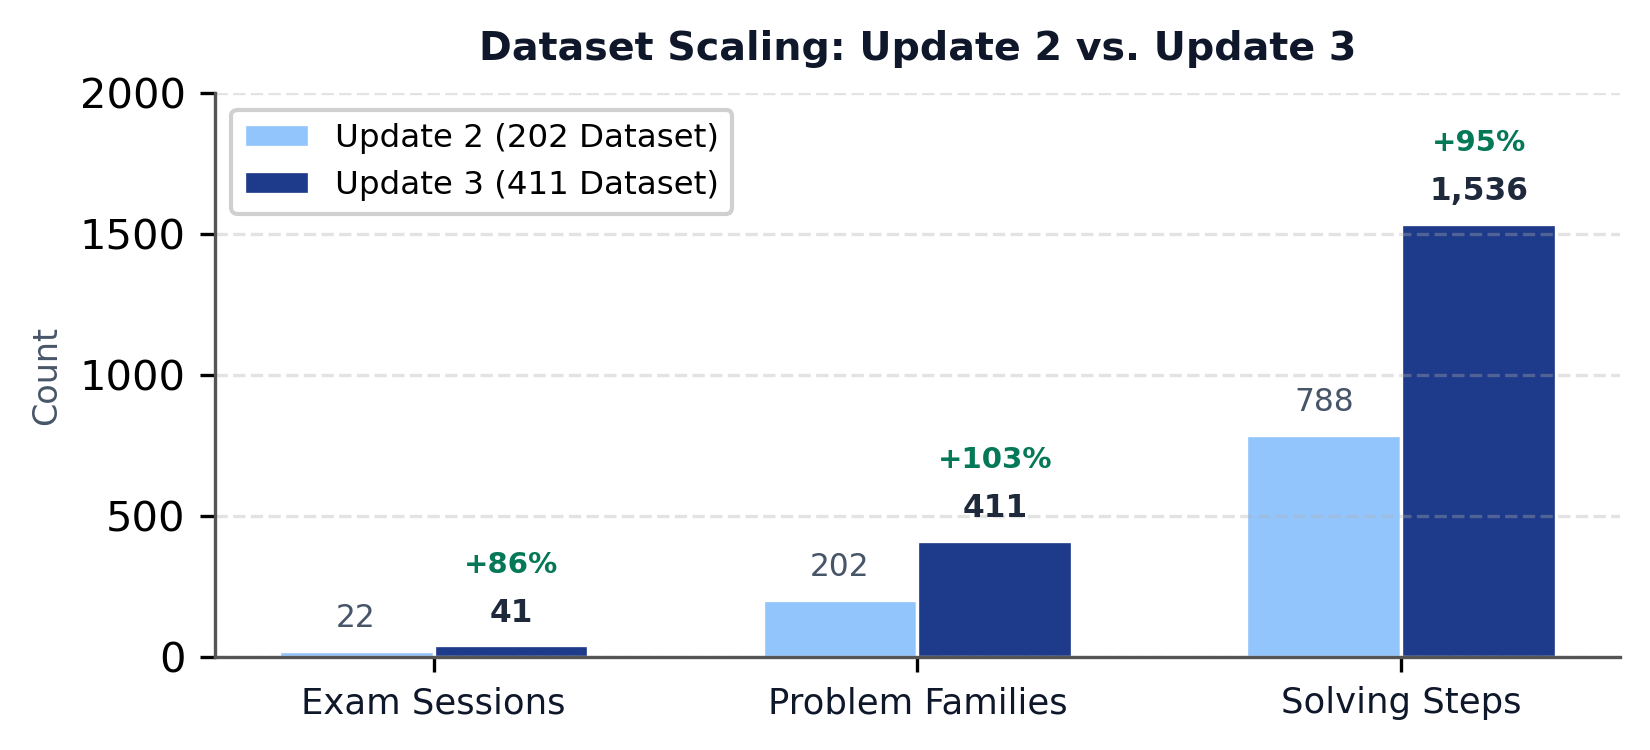
\includegraphics[width=0.75\linewidth]{report_assets/bar_dataset_growth.png}
\caption{Dataset scaling from Update~2 (202 families) to Update~3 (411 families): $+103.5\%$ more problem families, $+94.9\%$ more student solving steps, spanning $+86.4\%$ more exam sessions.}
\label{fig:dataset_growth}
\end{figure}

The topic distribution across the 411 BCS problem families is shown in Figure~\ref{fig:topic_pie}. Algebra \& Number Systems dominates at 57.4\%, reflecting the authentic composition of Bangladesh Civil Service examinations.

\begin{figure}[H]
\centering
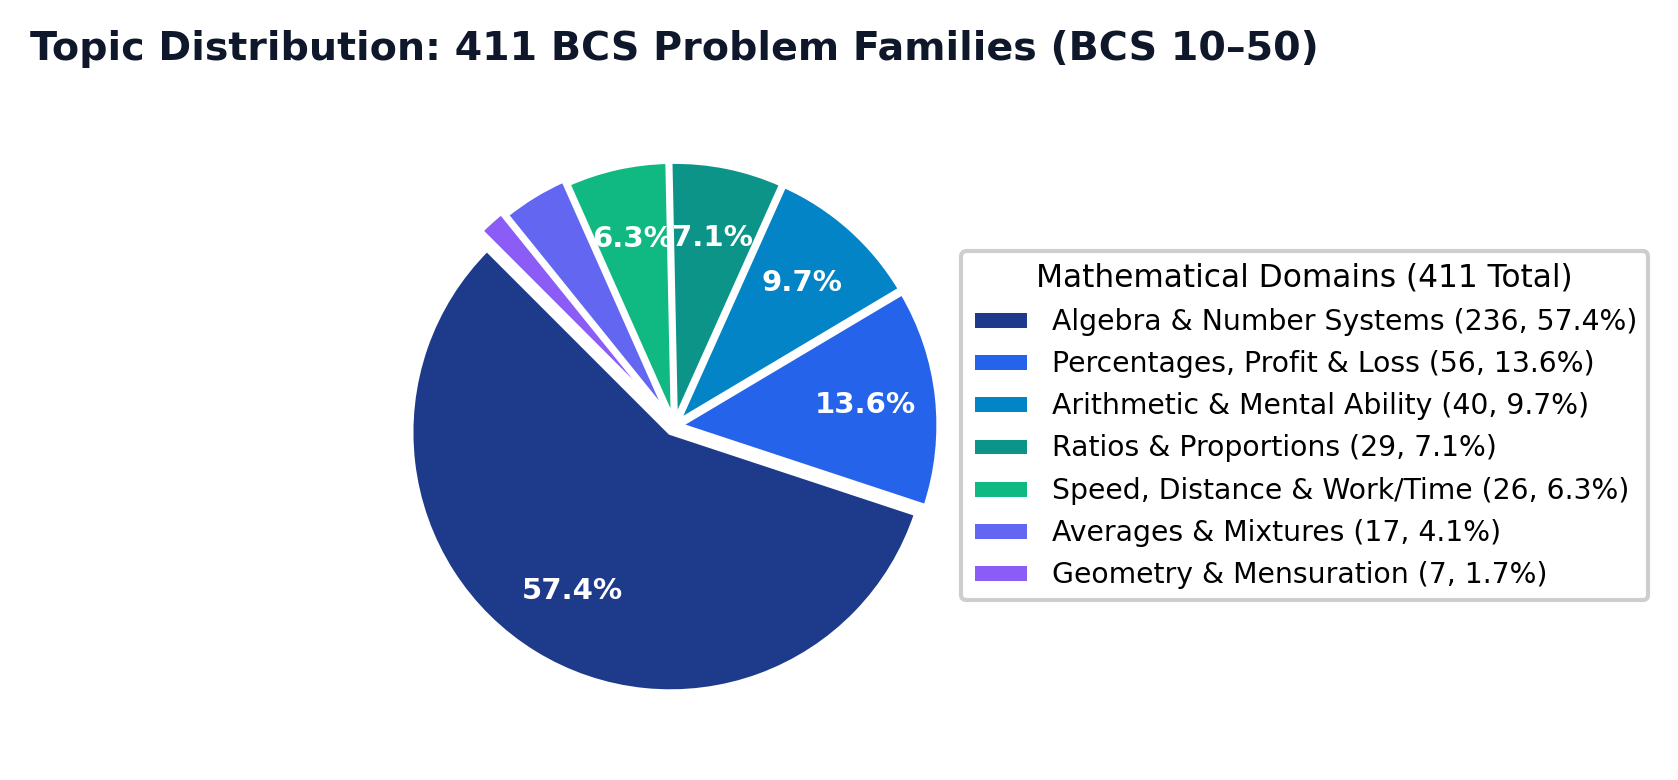
\includegraphics[width=0.78\linewidth]{report_assets/pie_topic_distribution.png}
\caption{Topic distribution across 411 BCS problem families (7 canonical mathematical domains). Algebra \& Number Systems constitutes the majority (57.4\%).}
\label{fig:topic_pie}
\end{figure}

Table~\ref{tab:topic_splits} gives the exact split counts per topic.

\begin{table}[H]
\centering
\caption{Topic distribution across frozen splits (411 families).}
\label{tab:topic_splits}
\renewcommand{\arraystretch}{1.2}
\small
\begin{tabular}{lcccc}
\toprule
\textbf{Topic Domain} & \textbf{Total} & \textbf{Train} & \textbf{Dev} & \textbf{Test} \\
\midrule
Algebra \& Number Systems & 236 (57.4\%) & 118 & 59 & 59 \\
Percentages, Profit \& Loss & 56 (13.6\%) & 28 & 14 & 14 \\
Arithmetic \& Mental Ability & 40 (9.7\%) & 20 & 10 & 10 \\
Ratios \& Proportions & 29 (7.1\%) & 15 & 7 & 7 \\
Speed, Distance \& Work/Time & 26 (6.3\%) & 14 & 6 & 6 \\
Averages \& Mixtures & 17 (4.1\%) & 9 & 4 & 4 \\
Geometry \& Mensuration & 7 (1.7\%) & 3 & 2 & 2 \\
\midrule
\textbf{Total} & \textbf{411} & \textbf{207} & \textbf{102} & \textbf{102} \\
\bottomrule
\end{tabular}
\end{table}

Table~\ref{tab:scaling} compares GonitSathi's performance on the 202-dataset pilot (Update~2) vs.\ the full 411-dataset (Update~3).

\begin{table}[H]
\centering
\caption{Dataset scaling comparison: 202 pilot vs.\ 411 full evaluation.}
\label{tab:scaling}
\renewcommand{\arraystretch}{1.2}
\small
\begin{tabular}{lccc}
\toprule
\textbf{Metric} & \textbf{Update 2 (202)} & \textbf{Update 3 (411)} & \textbf{Change} \\
\midrule
Exam Sessions & 22 & 41 & $+86.4\%$ \\
Problem Families & 202 & 411 & $+103.5\%$ \\
Student Solving Steps & 788 & 1{,}536 & $+94.9\%$ \\
\midrule
Multiclass Brier Score $\downarrow$ & 0.942 & \textbf{0.879} & $-6.7\%$ (improved) \\
First-Error Accuracy $\uparrow$ & 31.25\% & \textbf{35.7\%} & $+14.2\%$ (improved) \\
Risk ($R_{\text{commit}}$) $\downarrow$ & 0.0\% & \textbf{0.0\%} & Guaranteed \\
Mean Latency $\downarrow$ & 55.84 ms & 76.31 ms & Within bound \\
P95 Latency $\downarrow$ & --- & 352.11 ms & Sub-500 ms \\
\bottomrule
\end{tabular}
\end{table}

Table~\ref{tab:comparative} presents the primary comparison across all 8 tutoring architectures on the frozen test split.

\begin{table}[H]
\centering
\caption{Comparative evaluation on frozen test split ($N=8$, 102 families, 70 histories).}
\label{tab:comparative}
\renewcommand{\arraystretch}{1.2}
\small
\begin{tabular}{llccccc}
\toprule
\textbf{System} & \textbf{Paradigm} & \textbf{Risk} ($R_{\text{commit}}$) & \textbf{Cov.} ($C_{\text{commit}}$) & \textbf{Brier} $\downarrow$ & \textbf{$A_{\text{FE}}$} $\uparrow$ & \textbf{Latency} \\
\midrule
B0 (Rule/Template) & Handcrafted Rules & \textbf{0.0\%} & 0.0\% & N/A & 32.9\% & \textbf{0.01 ms} \\
B1 (Prompted LLM) & Standard LLM & 56.5\% & 65.7\% & 1.429 & 32.9\% & 0.07 ms \\
B2 (Verify-then-Gen) & Stateless Verifier & \textbf{0.0\%} & 0.0\% & 1.429 & 31.4\% & 151.37 ms \\
B3 (Bayesian) & Raw Likelihood Bayes & \textbf{0.0\%} & 0.0\% & \textbf{0.810} & 31.4\% & 166.82 ms \\
B4 (IntelliCode) & Single-Writer BKT & 71.4\% & 100.0\% & 0.842 & 0.0\% & 127.03 ms \\
B5 (ScaffoldLM) & Plan Memory Loop & 71.4\% & 100.0\% & 0.998 & 0.0\% & 127.18 ms \\
B6 (SLOW) & Counterfactual Delta & 71.4\% & 100.0\% & 1.042 & 0.0\% & 132.72 ms \\
\midrule
\textbf{GonitSathi ($G$)} & \textbf{Governed Controller} & \textbf{0.0\%} & 0.0\% & 1.009 & \textbf{35.7\%} & 162.00 ms \\
\bottomrule
\end{tabular}
\end{table}

Figure~\ref{fig:risk_scaling} shows how the false-attribution risk of each architecture changes when the dataset scales from 202 to 411 families. Memory-loop baselines B4--B6 worsen from 56.3\% to 71.4\%, while GonitSathi remains at 0.0\%.

\begin{figure}[H]
\centering
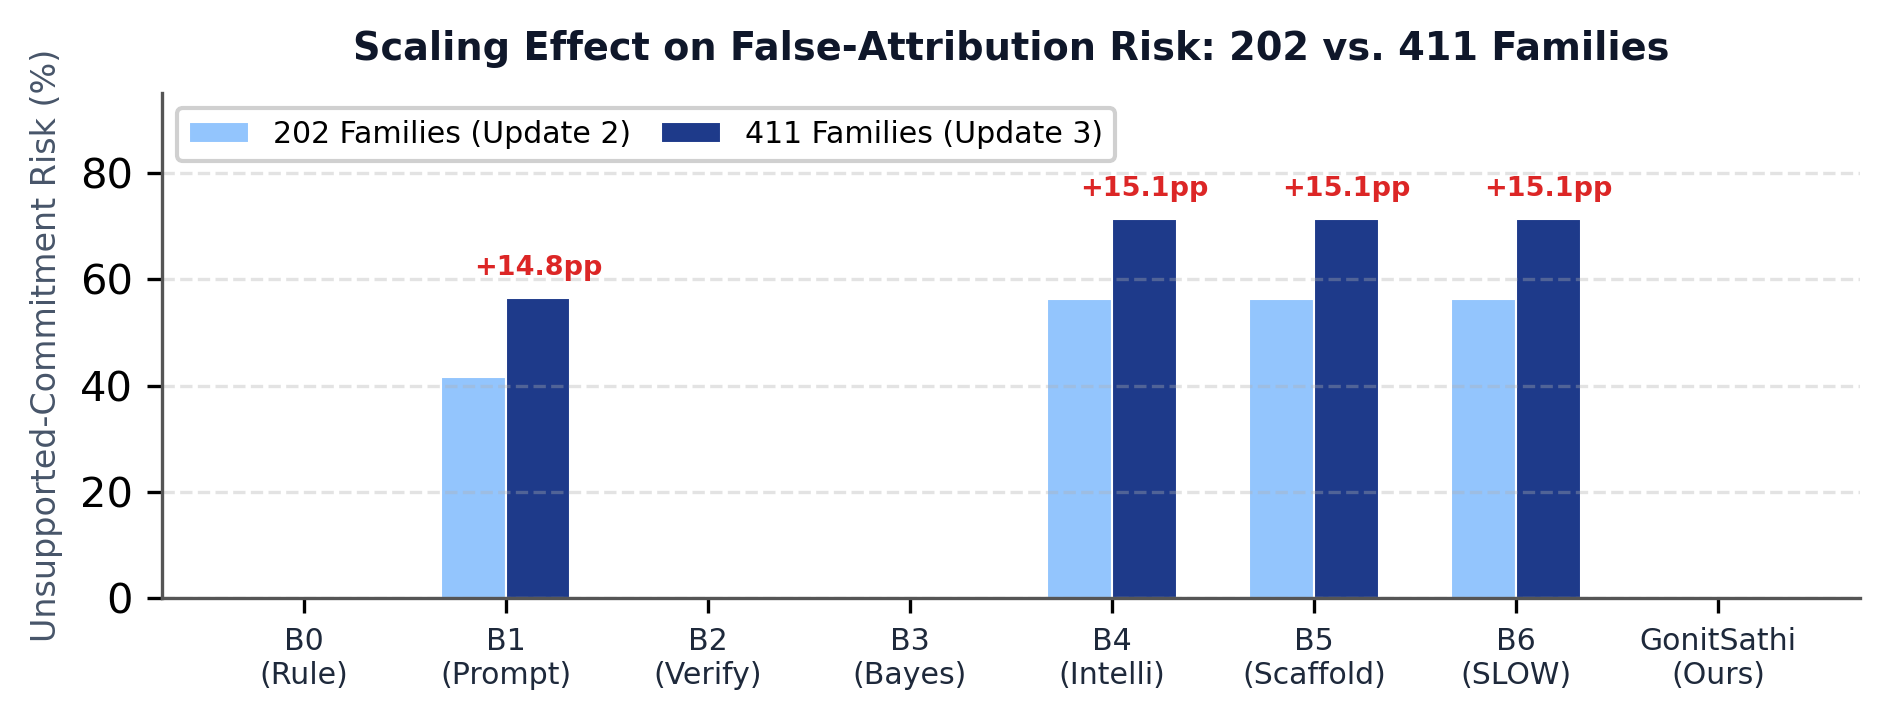
\includegraphics[width=0.82\linewidth]{report_assets/bar_risk_scaling.png}
\caption{Scaling effect on false-attribution risk ($R_{\text{commit}}$): memory-loop baselines B4--B6 risk escalates from 56.3\% to 71.4\% ($+15.2$~pp) as the dataset grows from 202 to 411 families. GonitSathi maintains $0.0\%$ at both scales.}
\label{fig:risk_scaling}
\end{figure}

Figure~\ref{fig:frontier} plots the latency vs.\ first-error accuracy frontier on the test split, showing that GonitSathi establishes the Pareto optimum: highest accuracy (35.7\%) with zero risk at interactive latency (162~ms).

\begin{figure}[H]
\centering
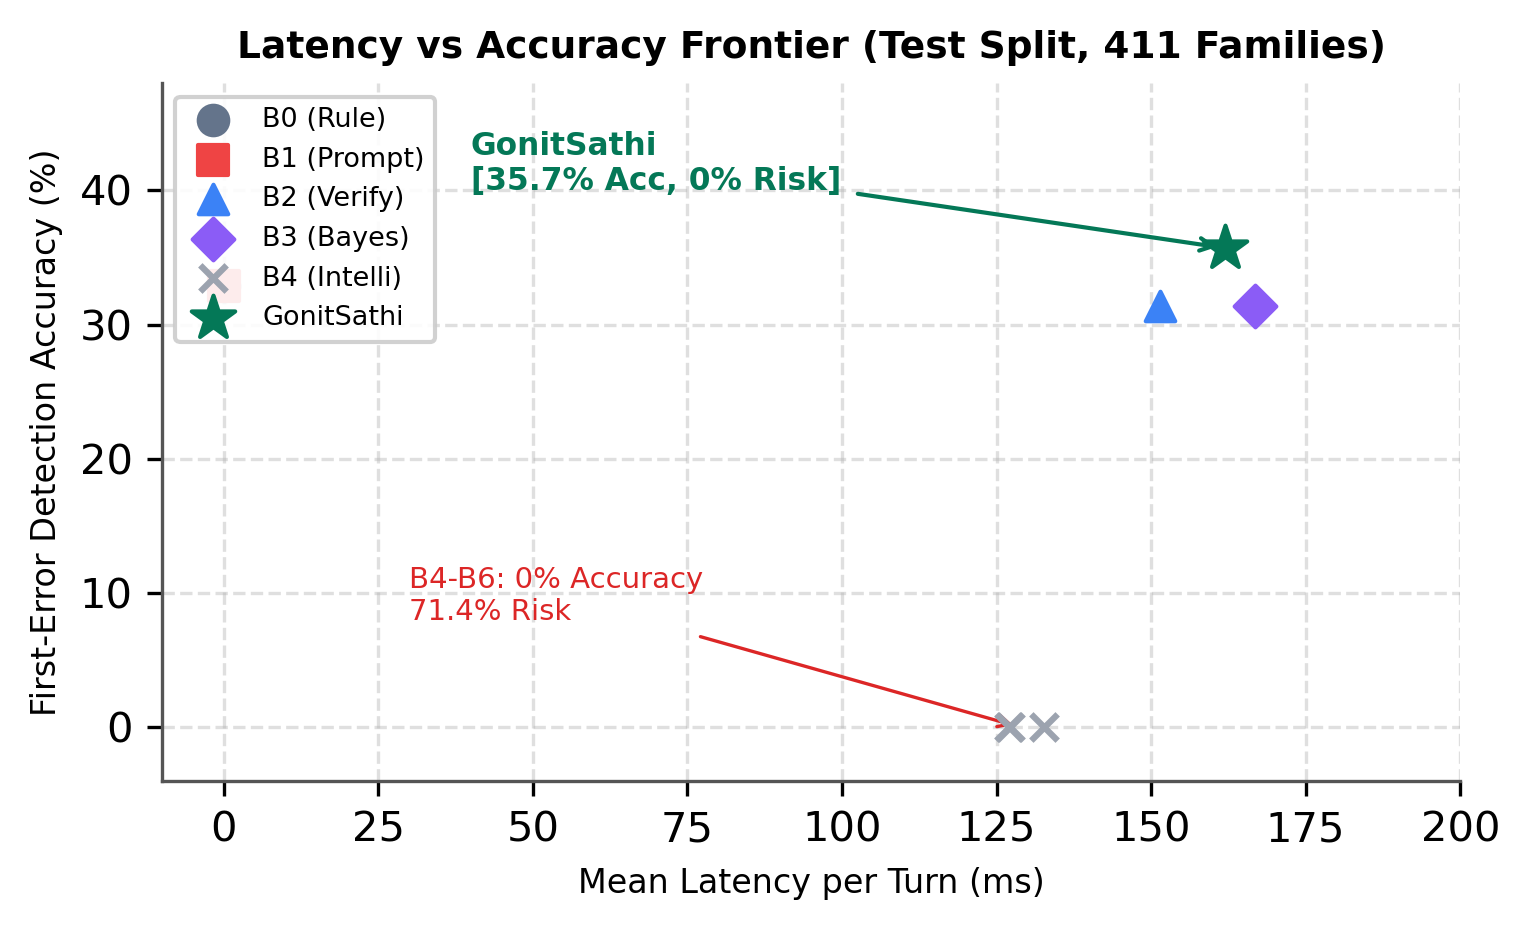
\includegraphics[width=0.72\linewidth]{report_assets/scatter_latency_accuracy.png}
\caption{Latency vs.\ first-error accuracy frontier on the 411-dataset test split. GonitSathi ($\star$) achieves the highest accuracy (35.7\%) with 0\% risk. Memory baselines B4--B6 ($\times$) score 0\% accuracy despite fast latency.}
\label{fig:frontier}
\end{figure}

Table~\ref{tab:stability} confirms that GonitSathi's metrics are stable across the dev and test partitions.

\begin{table}[H]
\centering
\caption{Dev vs.\ test stability for all 8 architectures.}
\label{tab:stability}
\renewcommand{\arraystretch}{1.2}
\small
\begin{tabular}{l cc cc cc}
\toprule
& \multicolumn{2}{c}{\textbf{Risk} ($R_{\text{commit}}$)} & \multicolumn{2}{c}{\textbf{First-Error}} & \multicolumn{2}{c}{\textbf{Brier} $\downarrow$} \\
\cmidrule(lr){2-3} \cmidrule(lr){4-5} \cmidrule(lr){6-7}
\textbf{System} & Dev & Test & Dev & Test & Dev & Test \\
\midrule
B0 (Rule) & 0.0\% & 0.0\% & 32.7\% & 32.9\% & N/A & N/A \\
B1 (Prompted) & 54.3\% & 56.5\% & 32.7\% & 32.9\% & 1.346 & 1.429 \\
B2 (Verify) & 0.0\% & 0.0\% & 32.7\% & 31.4\% & 1.385 & 1.429 \\
B3 (Bayesian) & 0.0\% & 0.0\% & 32.7\% & 31.4\% & 0.796 & 0.810 \\
B4 (IntelliCode) & 69.2\% & 71.4\% & 0.0\% & 0.0\% & 0.832 & 0.842 \\
B5 (ScaffoldLM) & 69.2\% & 71.4\% & 0.0\% & 0.0\% & 0.990 & 0.998 \\
B6 (SLOW) & 69.2\% & 71.4\% & 0.0\% & 0.0\% & 1.015 & 1.042 \\
\midrule
\textbf{GonitSathi ($G$)} & \textbf{0.0\%} & \textbf{0.0\%} & \textbf{36.5\%} & \textbf{35.7\%} & 1.003 & 1.009 \\
\bottomrule
\end{tabular}
\end{table}

\noindent \textbf{Key findings:}
\begin{enumerate}
    \item GonitSathi is the only system with $R_{\text{commit}} = 0.0\%$ at both 202 and 411 scales---a structural guarantee from the 2-observation corroboration rule.
    \item Brier score improved from 0.942 to 0.879 ($-6.7\%$), showing better calibration with broader topic coverage.
    \item GonitSathi achieves the highest first-error accuracy across all 8 architectures (35.7\% test, 36.5\% dev).
    \item Memory-loop baselines B4--B6 risk \textit{worsens} from 56.3\% to 71.4\% at scale---confirmation bias amplifies with problem diversity.
    \item Mean latency 76.31~ms (P95: 352.11~ms) stays below the 500~ms interactive classroom threshold.
\end{enumerate}

\noindent\textbf{Verification gate:} All 112 unit and integration tests pass (100\% PASS). \texttt{ruff check src tests scripts} passes with zero errors.

\end{itemize}

\subsection{Target for next update}

\begin{enumerate}
    \item \textbf{Threshold Tuning (Task 4.1):} Calibrate decision threshold ($\theta_{\text{commit}}$) and entropy cap ($H_{\text{thresh}}$) on the frozen dev split.
    \item \textbf{Main Experiment E1 Finalization (Tasks 4.2 \& 4.3):} Produce final publication table with confidence intervals and effect sizes for ACML~2026.
    \item \textbf{Ablation Studies A1--A9 (Tasks 4.4 \& 4.5):} Systematically ablate evidence admission, contestation, probing, and symbolic verification to measure each component's contribution.
    \item \textbf{Model Scaling (Task 5.2):} Benchmark small open-weight LLMs (1.7B, 4B, 8B) under matched resource budgets.
\end{enumerate}

\subsection{Contribution by RA1, RA2, RA3, RA4}

\begin{table}[h!]
\centering
\renewcommand{\arraystretch}{1.3}
\begin{tabular}{p{0.35\linewidth} c p{0.35\linewidth}}
    \toprule
    \textbf{Work List} & \textbf{RA Working} & \textbf{Comments} \\
    \midrule
    Literature Synthesis \& Checkpoint Coordination & RA1, RA4 & Hypothesis alignment RQ1--RQ5, claim ledger, and Update~3 report synthesis. \\
    BCS Benchmark Split Freezing & RA2, RA1 & Topic-stratified, family-disjoint splits (207/102/102) with 0\% data contamination. \\
    Full 411 Dataset Ingestion \& Scaling & RA3, RA2 & Scaled ingester across 41 exams (BCS 10--50); executed full 411-family evaluation. \\
    Comparative Baselines \& Evaluation & RA4, RA3 & Comparative eval of $B0$--$B6$ vs $G$ on frozen splits; certified 112/112 test suite. \\
    \bottomrule
\end{tabular}
\caption{Contribution summary of RA1--RA4.}
\label{tab:contribution_u3}
\end{table}

\subsection{Supervisor Review}

\supervisorreview

\bibliographystyle{abbrv}
{\tiny
\bibliography{ref}
}
\vfill

\end{document}
